\documentclass[12pt,a4paper]{article}
\usepackage[utf8]{inputenc}
\usepackage[T1]{fontenc}
\usepackage{fontspec}
\setmainfont{Times New Roman}
\newfontfamily\hackfont{Hack}
\usepackage{titlesec}
\usepackage{fancyhdr}
\usepackage{listings}
\usepackage{xcolor}
\usepackage{graphicx}
\usepackage{longtable}
\usepackage{caption}
\usepackage{hyperref}
\usepackage{setspace}
\usepackage{geometry}
\geometry{a4paper, margin=1in}
\hypersetup{colorlinks=true, linkcolor=blue, urlcolor=blue}
\renewcommand{\contentsname}{Table of Contents}

\pagestyle{fancy}
\fancyhf{} 							% Header Middle
\rhead{VLSI Design Lab}
\lhead{Lab-06: Stick Diagram of XOR Gate}
\rfoot{\thepage}

\begin{document}

\begin{titlepage}					% Cover Start
\begin{center}
    
\includegraphics[width=0.35\textwidth]{logo.png} \\
    \vspace{0.5cm}
    \textbf{\Huge \textcolor{cyan}{NOTRE DAME} \textcolor{cyan}{UNIVERSITY}} \\
    \vspace{0.5cm}
    \textbf{\Huge \textcolor{orange}{BANGLADESH}} \\
    
    \vspace{0.9cm}
    \textbf{\Huge \underline{VLSI Design Lab Report-06}} \\
    
    \vspace{1.5em}
    \begin{flushleft}
    	\textbf{\Large Course Code: CSE-4218} \\
		\vspace{0.3cm}        
        \textbf{\Large Course Title: VLSI Design Lab} \\
        \vspace{0.3cm}
        \textbf{\Large Experiment Name: Stick Diagram of XOR Gate} \\        
    \end{flushleft}
    
    \vspace{1em}
    \begin{flushleft}
        \textbf{\Huge \textcolor{blue}{Submitted by:}} \\
        \vspace{0.3cm}
        \textbf{\Large Name: Istiak Alam} \\
        \vspace{0.3cm}
        \textbf{\Large ID: 0692230005101005} \\
		\vspace{0.3cm}        
        \textbf{\Large Batch: CSE-20} \\
        \vspace{0.5cm}
        \textbf{\Large Submission Date: }{\Large \textbf{\today}\par}
    \end{flushleft}
    \vfill
    \begin{flushleft}
        \textbf{\Huge \textcolor{blue}{Submitted to:}} \\
        \vspace{0.3cm}
        \textbf{\Large Nafisa Tabassum,} \\
        \vspace{0.3cm}
        \textbf{\Large Lecturer, Dept. of CSE} \\
        \vspace{0.3cm}
        \textbf{\Large Notre Dame University Bangladesh}
    \end{flushleft}
\end{center}
\end{titlepage}						% Cover End

\tableofcontents
\thispagestyle{empty}
\clearpage
\pagenumbering{arabic}

\section*{\center Abstract}
This laboratory experiment presents the implementation of the stick diagram of an XOR gate using the Microwind2 layout design tool. The XOR gate was realized based on its Boolean expression and CMOS logic principles. A simplified stick diagram was developed using standard layer representations such as polysilicon, diffusion, and metal interconnections. The functionality of the design was verified through simulation, and the output waveform was analyzed to confirm correct logical behavior. The experiment provides a clear understanding of the relationship between Boolean functions, CMOS circuit design, and their physical layout representation in VLSI systems.




\section{Introduction}
In VLSI design, the transformation of logical circuits into physical layouts is an essential step in the design process. Stick diagrams serve as a simplified and technology-independent method for representing circuit layouts, allowing designers to visualize transistor placement and interconnections without focusing on exact dimensions.

The XOR gate is an important combinational logic circuit widely used in arithmetic and digital systems. Its implementation in CMOS requires careful arrangement of pull-up and pull-down networks. In this experiment, the XOR gate is designed using its Boolean expression and represented using a stick diagram in Microwind2. The study of this design helps in understanding layout organization, layer interaction, and efficient circuit realization in VLSI systems.



\section{Objective}
The objectives of this laboratory experiment are as follows:
\begin{itemize}
    \item To understand the concept and importance of stick diagrams in VLSI layout design.
    \item To implement stick diagrams of basic CMOS logic gates using Microwind2.
    \item To represent transistor-level circuits using simplified, technology-independent layouts.
    \item To analyze the arrangement of polysilicon, diffusion, and metal layers in CMOS design.
    \item To develop a clear understanding of the relationship between schematic design and physical layout.
\end{itemize}


\newpage
\section{XOR Gate}

An XOR (Exclusive-OR) gate is a combinational logic gate that produces a logic HIGH output when the inputs are different and a logic LOW output when the inputs are the same. It is commonly used in digital circuits for comparison, parity checking, and arithmetic operations. 

\subsection*{Boolean Function}
\[
Y = (AB+A'B')'
\]

\subsection*{Truth Table}
\begin{center}
\begin{tabular}{|c|c|c|}
\hline
A & B & Y \\ \hline
0 & 0 & 0 \\
0 & 1 & 1 \\
1 & 0 & 1 \\
1 & 1 & 0 \\ \hline
\end{tabular}
\end{center}

\subsection*{Stick Diagram}
\begin{figure}[!h]
\centering
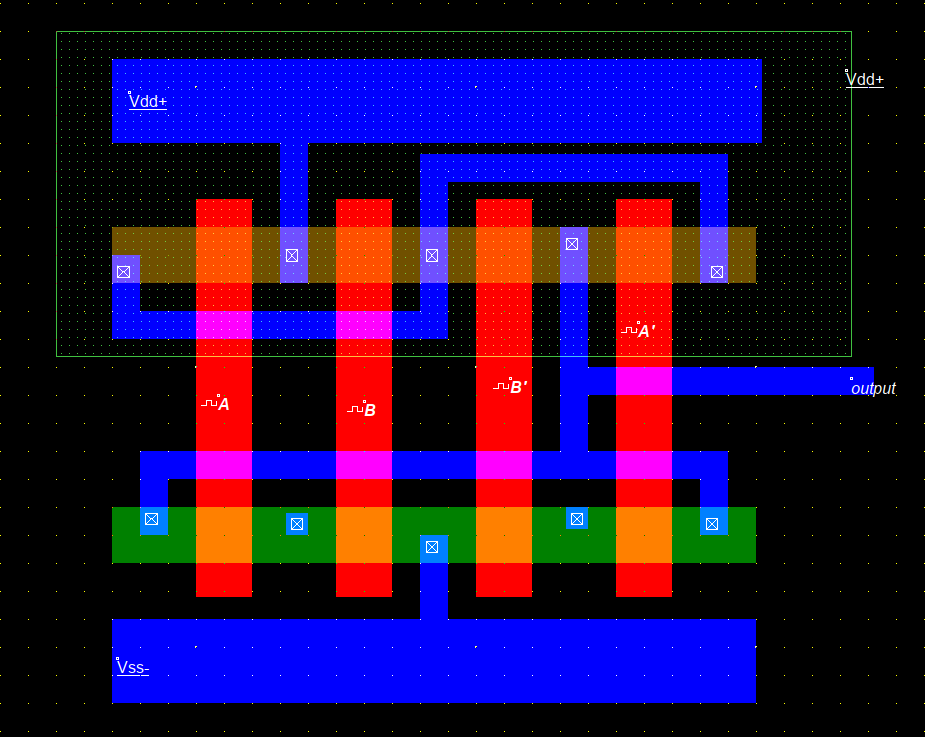
\includegraphics[width=0.7\textwidth]{XOR-Function-Stick-Diagram.png}
\caption{Stick Diagram of XOR Gate}
\end{figure}
\newpage
\subsection*{Output}
\begin{figure}[!h]
\centering
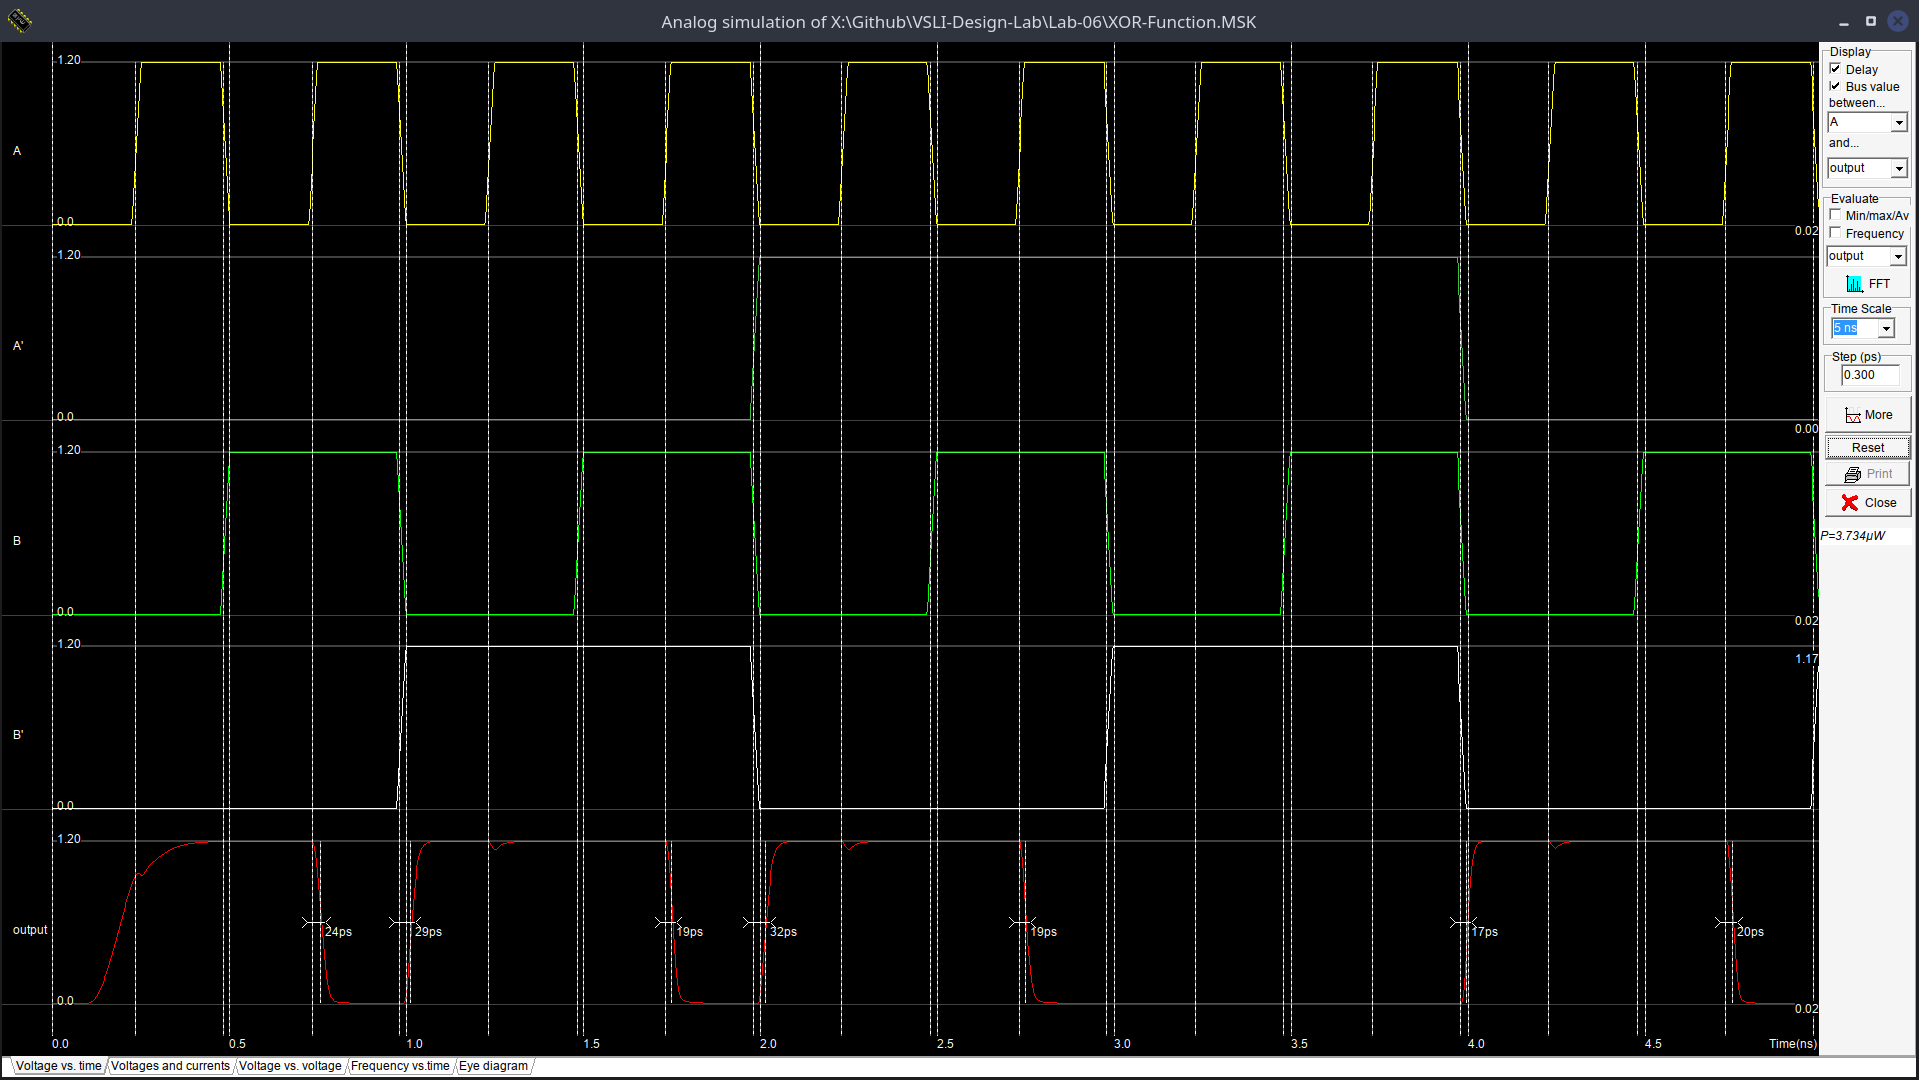
\includegraphics[width=1\textwidth]{XOR-Function-Output.png}
\caption{Output in Analog Simulation of XOR Gate}
\end{figure}

\subsection*{Observation}
From the implementation and simulation of the XOR gate stick diagram using Microwind2, it was observed that the circuit produces a logic HIGH output when the inputs are different and a logic LOW output when both inputs are the same. The output waveform obtained from the simulation matches the theoretical truth table of the XOR function.

The stick diagram correctly represents the CMOS structure using appropriate placement of polysilicon, diffusion, and metal layers. Proper alignment and interconnection of these layers ensured correct signal flow and circuit operation. The simulation results confirm that the designed layout accurately implements the XOR logic function.



% =====================================================
\section{Conclusion}
In this laboratory experiment, the stick diagram of an XOR gate was successfully designed and implemented using Microwind2. The experiment demonstrated how a Boolean expression can be translated into a CMOS-based layout representation using simplified stick diagram techniques.

The simulation results verified that the implemented design functions correctly according to the XOR truth table. This experiment enhanced the understanding of CMOS layout design, layer organization, and the relationship between logical design and physical implementation. The knowledge gained from this lab is essential for advanced VLSI design and layout optimization.





\end{document}